\documentclass[a4paper,slidestop,xcolor=pst,blue]{beamer}

\usepackage{beamerthemesplit}
\usepackage[utf8]{inputenc}
\usepackage[spanish]{babel}
\usepackage{graphicx}
\usepackage{pstricks} % PSTricks package
\usepackage{setspace}
\usepackage{multirow}
\usepackage{listings}
\usepackage{pgfpages}
\usepackage{hyperref}
\usepackage{etoolbox}
\usepackage{epstopdf}

\makeatletter
\patchcmd{\beamer@sectionintoc}{\vskip1.5em}{\vskip0.5em}{}{}
\makeatother

\setbeamercovered{dynamic}
\setcounter{tocdepth}{2}
\setbeamercolor{frametitle}{fg=black,bg=white}
\setbeamercolor{section in toc shaded}{fg=black}
\setbeamercolor{section in toc}{fg=red}
\setbeamercolor{subsection in toc shaded}{fg=black}
\setbeamercolor{subsection in toc}{fg=red}
\setbeamerfont{section in toc}{size=\small}
\setbeamerfont{subsection in toc}{size=\small}
\setbeamertemplate{section in toc shaded}[default][99]
\setbeamertemplate{subsection in toc shaded}[default][99]

\AtBeginSection[]
{\begin{frame}[c]
  \frametitle{Índice}
	\tableofcontents[currentsection,
        sectionstyle=show/shaded,
        subsectionstyle=hide]
\end{frame}}

\AtBeginSubsection[]
{\begin{frame}[c]
	\frametitle{Índice}
	\tableofcontents[
  		currentsection,
  		sectionstyle=shaded/shaded,
  		currentsubsection,
  		subsectionstyle=show/shaded/hide
		]
\end{frame}}

\setbeamercolor{frametitle}{fg=black,bg=white}

\setbeamertemplate{frametitle}{
	\begin{centering}
		\insertframetitle
		\par
	\end{centering}
}

\usetheme[secheader]{Boadilla} 
\usepackage{listings}

\definecolor{pblue}{rgb}{0.13,0.13,1}
\definecolor{pgreen}{rgb}{0,0.5,0}
\definecolor{pred}{rgb}{0.9,0,0}
\definecolor{pgrey}{rgb}{0.46,0.45,0.48}

\lstset{language=Java,
  showspaces=false,
  showtabs=false,
  breaklines=true,
  showstringspaces=false,
  breakatwhitespace=true,
  commentstyle=\color{pgreen},
  keywordstyle=\color{pblue},
  stringstyle=\color{pred},
  basicstyle=\ttfamily,
  keywordsprefix={@}
}


\newcommand{\ann}[1]{\color{blue}\texttt{#1}\color{black}}

\title[Rest Controllers]{Capa de Servicio \\ Spring Rest Controllers y Soporte para Transacciones}

\author[P. S{\'a}nchez]{\alert{Pablo S{\'a}nchez}}

\institute[IIE]{
		   Dpto. Ingenier{\'i}a Inform{\'a}tica y Electr{\'o}nica \\
		   Universidad de Cantabria \\
		   Santander (Cantabria, Espa{\~n}a) \\
		   \texttt{p.sanchez@unican.es}
}

\date{}

\begin{document}

\begin{frame}[c]
	\titlepage
	\begin{columns}
		\column{0.50\linewidth}
			\centering
    		
\includegraphics[width=.28\textwidth,keepaspectratio=true]{images/istr.eps}
		\column{0.50\linewidth}
			\centering
			
\includegraphics[width=.25\textwidth,keepaspectratio=true]{images/uc.eps}
	\end{columns}
\end{frame}

\begin{frame}[c]
    \frametitle{\alert{Advertencia}}
    \begin{center}
        Todo el material contenido en este documento no constituye en modo alguno una obra de referencia o apuntes oficiales mediante el cual se puedan preparar las pruebas evaluables necesarias para superar la asignatura. \ \\
        \ \\
        Este documento contiene exclusivamente una serie de diapositivas cuyo objetivo es servir de complemento visual a las actividades realizadas en el aula para la transmisi{\'o}n del contenido sobre el cual versar{\'a}n las mencionadas pruebas evaluables.  \ \\
        \ \\
        Dicho de forma m{\'a}s clara, \alert{estas transparencias no son apuntes y su objetivo no es servir para que el alumno pueda preparar la asignatura.}
    \end{center}
\end{frame}

\section{Introducción}

\begin{frame}[c]
    \frametitle{Objetivos del Tema}
    \begin{enumerate}[<+->]
         \item Ser capaz de crear controladores REST utilizando \emph{Spring}.
         \item Ser capaz de especificar cómo serializar POJOs usando \emph{Jackson}.
         \item Ser capaz de especificar transaccionalidad usando \emph{Spring}.
    \end{enumerate}
\end{frame}

%\begin{frame}[c]
%    \frametitle{Bibliografía}
%    \begin{thebibliography}{1}
%
%        \bibitem[Spring, 2019]{Spring2019}
%        \em {Spring Reference Documentation}.
%        \newblock{\url{https://goo.gl/AzsbtY}}
%
%    \end{thebibliography}
%\end{frame}

\begin{frame}[c]
    \frametitle{Arquitectura MVC}
    \begin{center}
        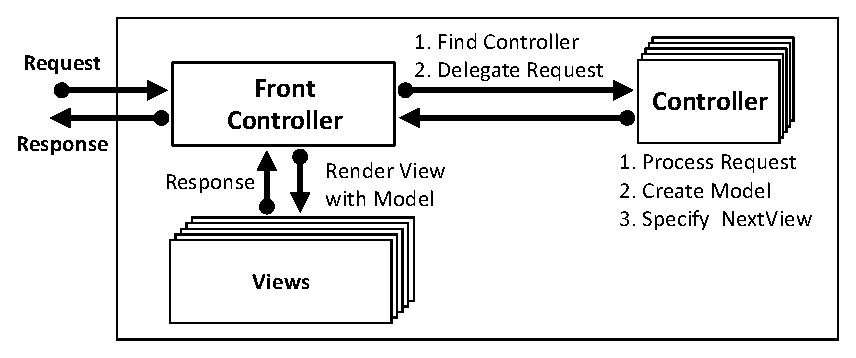
\includegraphics[width=\linewidth,keepaspectratio=true]{images/mvc/mvc00.eps}
    \end{center}
\end{frame}

\section{Spring Rest Controllers}

\begin{frame}[c]
    \frametitle{Anotaciones Rest}
    \begin{tabular}{lp{0.70\linewidth}}
        \ann{@RestController} &  La clase contendrá controladores REST. \\
        \ann{@RequestMapping} &  URI raíz asociada a un \texttt{RestController}. \\
        \ann{@GetMapping}     &  Controlador GET (de la URI correspondiente).  \\
        \ann{@PostMapping}    &  Controlador POST (de la URI correspondiente). \\
        \ann{@PutMapping}     &  Controlador PUT (de la URI correspondiente). \\
        \ann{@DeleteMapping}  &  Controlador DELETE (de la URI correspondiente). \\
        \ann{@PathVariable}   &  El parámetro se extrae de una variable de la URI. \\
        \ann{@RequestParam}   &  Parámetros de la petición HTTP. \\
        \ann{@RequestBody}    &  Parámetro enviado en el cuerpo de la petición \\
    \end{tabular}
\end{frame}

\begin{frame}[c,fragile]
    \frametitle{Respuestas HTTP}
    \begin{lstlisting}[basicstyle=\small,language=Java]
@GetMapping(value="usuarios/{id}")
public ResponseEntity<Usuario>
        obtenerUsuario(@PathVariable("id")
                              String userId) {

   Optional<Usuario> u = ur.findById(userId);
   ResponseEntity<Usuario> result;
	
   if (u.isPresent()) {
     result = ResponseEntity.ok(u.get());
   } else {
     result = ResponseEntity.notFound().build();
   }

   return result; 	
}
\end{lstlisting}
\end{frame}

\section{Jackson}

\subsection{Anotaciones básicas}

\begin{frame}[c]
    \frametitle{Anotaciones Jackson}
    %% Se mapea todo aquello que tenga getter.
    \begin{tabular}{lp{0.70\linewidth}}
        \ann{@JsonAutoDetect} & Define qué se serializa (e.g. público) \\
        \ann{@JsonProperty}   & \\
        \multicolumn{1}{c}{\ann{(``nombre'')}} & El elemento se mapeará con el nombre indicado. \\
        \ann{@JsonIgnore}     & El elemento se ignora. \\
        \ann{@JsonUnwrapped}  & El objeto se mapea como campos del contenedor. \\
        \ann{@JsonValue}      & Sólo se mapea el valor de este elemento. \\
        \ann{@JsonManaged}    &  \\
        \multicolumn{1}{c}{\ann{Reference}} & Padre en referencia bidireccional padre-hijo.  \\
        \ann{@JsonBack}       &    \\
        \multicolumn{1}{c}{\ann{Reference}} & Hijo en referencia bidireccional padre-hijo.  \\
    \end{tabular}
\end{frame}

\subsection{Vistas}

\begin{frame}[c,fragile]
    \frametitle{Vistas Jackson - Definición}
\begin{lstlisting}[basicstyle=\small,language=Java]
public class Views {

  public static class DescripcionViaje {};
  public static class DescripcionUsuario {}

}
\end{lstlisting}
\end{frame}

\begin{frame}[c,fragile]
    \frametitle{Vistas Jackson - Selección de Propiedades}
\begin{lstlisting}[basicstyle=\small,language=Java]
public class Usuario {
	
  @Id
  @JsonView({Views.DescripcionViaje.class,
             Views.DescripcionUsuario.class})
  protected String username;
  @JsonView({Views.DescripcionUsuario.class})
  protected String nombre;
  @JsonView({Views.DescripcionUsuario.class})
  protected String apellido;
  @JsonView({Views.DescripcionUsuario.class})
  protected String email;

}
\end{lstlisting}
\end{frame}

\begin{frame}[c,fragile]
    \frametitle{Vistas Jackson - Controlador Rest}
\begin{lstlisting}[basicstyle=\small,language=Java]
@GetMapping("/{viajeId}")
@JsonView(Views.DescripcionViaje.class)
public ResponseEntity<Viaje>
                getViaje(@PathVariable Long viajeId) {}
\end{lstlisting}
\end{frame}

\section{Soporte para Transacciones Spring JPA}

\subsection{Elementos de una Transacción JPA}

\begin{frame}[c]
    \frametitle{Elementos Transaccionales JPA}
    \begin{center}
        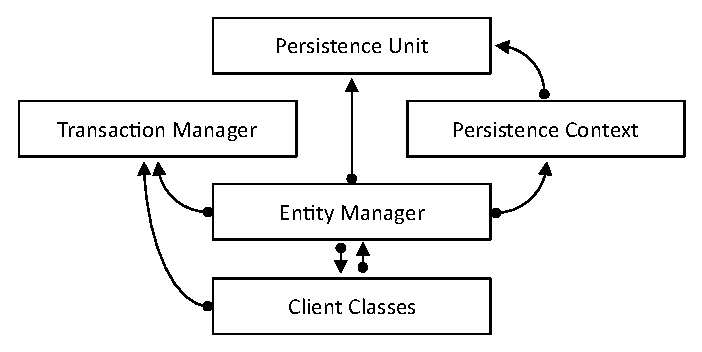
\includegraphics[width=0.8\linewidth,keepaspectratio=true]{images/jpa/jpaElements.eps}
    \end{center}
\end{frame}

\subsection{Ciclo de Vida de una Entidad JPA}

\begin{frame}[c]
    \frametitle{Ciclo de Vida de una Entidad}
%    \begin{center}
%        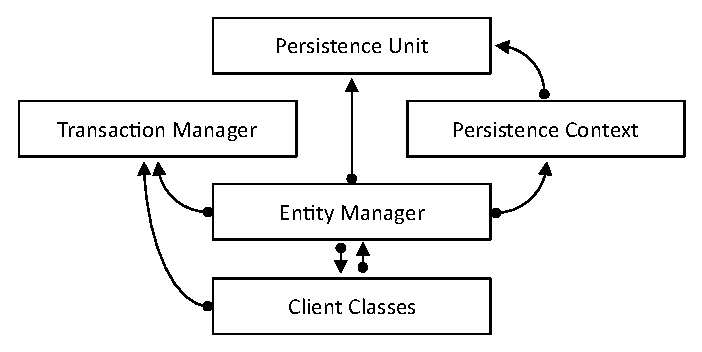
\includegraphics[width=0.8\linewidth,keepaspectratio=true]{images/jpa/jpaElements.eps}
%    \end{center}
\end{frame}

\begin{frame}[c]
    \frametitle{Interfaz Entity Manager}
    \begin{tabular}{lp{0.70\linewidth}}
        persist(Object ent)    & Registra una entidad como nueva \\
        remove(Object entity)  & Anota una entidad para su eliminación.    \\
        find(Class type, Object id) & Carga una entidad desde persistencia. \\
        detach(Object entity)  & Carga una entidad desde persistencia. \\
        merge(Object entity)   & Anota una entidad para su actualización.  \\
        refresh(Object entity) & Actualiza una entidad en el \emph{identity map}. \\
        flush()                & Guarda los cambios en persistencia. \\
    \end{tabular}
\end{frame}

\subsection{Anotaciones \emph{Entity Manager}}

\begin{frame}[c]
    \frametitle{Anotaciones \emph{Entity Manager}}
    \begin{tabular}{lp{0.70\linewidth}}
        \ann{@PersistenceUnit}    & Inyecta una \emph{Entity Manager Factory} \\
        \ann{@PersistenceContext} & Inyecta un \emph{Entity Manager} \\
    \end{tabular}
\end{frame}

\subsection{Métodos Transaccionales}

%% Método largo, con entity manager inyectado
%% Anotacion Transactional

\section{Sumario}

\begin{frame}[c]
    \frametitle{¿Qué tengo que saber de todo ésto?}
    \begin{enumerate}[<+->]
        \item Ser capaz de utilizar anotaciones \emph{Spring MVC} para implementar controladores Rest.
        \item Ser capaz de utilizar anotaciones \emph{Jackson} para serializar POJOs a JSON.
        \item Comprender el funcionamiento del \emph{Entity Manager}.
        \item Ser capaz de utilizar anotaciones para definir transacciones en \emph{Spring}.
    \end{enumerate}
\end{frame}

\end{document}
